\section{Patterns im Kontext}

Die vorgestellten Concurrency Modelle und die Reactive Design Patterns sind Bausteine für die Entwicklung von reaktiven Systemen im Sinne des Reactive Manifestos. In diesem Abschnitt werden die Concurrency Modelle sowie die einzelnen Reactive Design Patterns in Zusammenhang gebracht. Dies soll gleichermaßen einen Überblick verschaffen und deren Verwendungszweck durch Klassifierung verdeutlichen.\\
Das Reactive Manifesto beschreibt vier Eigenschaften unter deren Gesichtspunkten, die Design Patterns eingeordnet werden. Um die Patterns im Kontext des Reactive Manifestos zu klassifizieren, werden die Eigenschaften nochmals auf deren Kern hin beschrieben.\\

Die grundlegende Eigenschaft \textit{message-driven} besagt, dass die Anwendung asynchronen Nachrichtenaustausch der synchronen Kommunikation vorziehen soll. Dies schafft die Möglichkeit einer lose Kopplung zwischen den Kommunikationsteilnehmern und macht diese weniger voneinander abhängig. Außerdem ermöglicht die nachrichtenbasierte Kommunikation eine Vielzahl von Design Patterns, wie sie beispielsweise in den Büchern \enquote{Enterprise integration patterns} von Hophe und Woolf oder \enquote{Reactive messaging patterns with Actor model} von Vernon beschrieben werden.\\
Die lose Kopplung der Komponenten ist auch für die Eigenschaft \textit{elastic} von Bedeutung. Die Eigenschaft besagt, dass die Anwendung dynamisch je nach Last skalieren muss. Dies bezieht sich sowohl auf die Skalierung einer Komponente auf einem Host als auch auf die Skalierung einer Komponente über mehrere Hosts hinweg. Um dies zu ermöglichen, müssen die Komponenten voneinander isoliert sein, sodass sie unabhängig skalieren können. Erst mithilfe der Isolation wird eine lose Kopplung realisierbar. Zusätzlich ist ein geeignetes Concurrency Modell nötig, um die Skalierung effizient und wartungsarm zu ermöglichen.\\
Die Isolation erfolgt nicht nur auf funktionaler Ebene. Für die Eigenschaft \textit{resilient} ist es nötig, die Komponenten gegen kaskadierende Fehler abzuschirmen. Zudem werden beim Entwurf von reaktiver Software von vornherein Fehlerzustände mit eingeplant. Dies erfordert wiederum ein umfangreiches Failure Management.\\
Das Ziel von alle dem ist eine Software, die auf jegliche Anfrage in angemessener Zeit reagiert. Dieses Ziel wird in der vierten und letzten Eigenschaft \textit{responsive} formuliert. Dazu ist es nötig maximale Antwortzeiten zu definieren.\\

Um die Patterns in Kontext zueinander setzen zu können, werde diese in der folgenden Abbildung (\ref{fig:patterns-context}) gruppiert dargestellt. Die Gruppen ergeben sich aus den Anforderungen, die sich aus den vier reaktiven Eigenschaften heraus gebildet haben. Jeder dieser Gruppen werden Reactive Design Patterns sowie weitere Randbedingungen zugeordnet. Die Gruppen lauten: \textbf{Isolation}, \textbf{Loose Coupling}, \textbf{Failure Management}, \textbf{Latency Control}, \textbf{Concurrency}.

\subsection{Isolation}
Die Isolation von Komponenten erfolgt auf funktionaler Ebene und zum Schutz vor kaskadierenden Fehlern. Sie wird durch die reaktiven Eigenschaften \textit{elastic} und \textit{resilient} vorgeschrieben. Das aus dem Single Responsibilty Principle hervorgehende Simple Component Pattern (\ref{subsec:simple-component-pattern}) ist somit ein grundlegendes Pattern. Das zu Beginn erwähnte Share nothing Prinzip (\ref{subsec:sharenothing}) schlägt ebenfalls in diese Kerbe --- auch wenn sich die Motivation hinter Share nothing auf Concurrency bezieht. Das Bulkheads Pattern (\ref{subsec:bulkheads-pattern}) schützt vor kaskadierenden Fehlern durch beispielsweise redundante Hardware oder durch separate Connection Pools. Die Patterns zur Isolation sollten grundsätzliche schon während des Entwurfs herangezogen werden. Es ist schwierig, zu einem späteren Zeitpunkt die Isolation von Komponenten in einem System herzustellen.

\subsection{Loose Coupling}
Die lose Kopplung von Komponenten wird durch die Isolation und die asynchrone Nachrichtenübertragung ermöglicht. Der Sender wird im Vergleich zur synchronen Kommunikation vom Empfänger entkoppelt. Der Sender kann unabhängig von der Verarbeitungsgeschwindigkeit weitere Aktionen durchführen, da dieser nicht auf dessen Antwort warten muss. Wie auch die Isolation wird die lose Kopplung von den reaktiven Eigenschaften \textit{elastic} und \textit{resilient} vorgeschrieben. Das mehrmals erwähnte Prinzip der Location Transparency ist hierfür relevant. Erst wenn die verteilten Komponenten unabhängig von deren Konstellation und Verteilung miteinander agieren können, wird die dynamische Skalierung ermöglicht. Ebenso spielt das Idempotent Receiver Pattern (\ref{subsec:idempotent-receiver-pattern}) eine Rolle, da die Verarbeitung von nicht idempotenten Aktionen in einem verteilten System schwieriger ist und die Kopplung erhöht.

\subsection{Failure Management}
In verteilten Systemen sind unvorhersehbare Fehlerzustände unvermeidbar. Zudem sind fehlerfreie Software Systeme nahezu unmöglich und meist mit unwirtschaftlichem Aufwand verbunden. Um dennoch die Eigenschaft \textit{resilient} erfüllen zu können, müssen Fehlerzustände von vornherein bedacht werden. Die Hierarchie der Komponenten --- entstanden durch das Simple Component Pattern --- ermöglicht das Prinzip der Supervision. Jede Komponente ist in der Verantwortung bei Fehlerzuständen der Unterkomponenten entsprechend zu reagieren oder zu eskalieren. Hierbei helfen die Patterns Heartbeat (\ref{subsec:heartbeat-pattern}) und Let-It-Crash (\ref{subsec:let-it-crash-pattern}). Das Prinzip Graceful Degradation of Service kann mit dem Fallback Pattern umgesetzt werden. Außerdem werden mit dem Fallback Pattern (\ref{subsec:fallback-pattern}) und dem Saga Pattern (\ref{subsec:saga-pattern}) Ausweichstrategien und ausgleichende Maßnahmen definiert, welche zur \textit{resilience} beitragen. Anders als verteilte Transaktionen entkoppelt das Saga Pattern die kommunizierenden Komponenten.

\subsection{Latency Control}
Für die \textit{responsiveness} müssen Timeouts und weiche Echtzeitanforderungen definiert werden. Um diese einzuhalten wird auf die Patterns Circuit Breaker (\ref{subsec:circuit-breaker-pattern}) und Fail Fast (\ref{subsec:fail-fast-pattern}) zurückgegriffen. 

\subsection{Concurrency}
Neben der grundlegenden Eigenschaft \textit{message-driven} ist ein effizientes Concurrency Modell für die \textit{elasticity} wesentlich. Die zwei vorgestellten Modelle der ereignisbasierten Concurrency (\ref{subsec:eventdriven-concurrency}) und der Actor-basierten Concurrency (\ref{subsec:actor-model}) eigenen sich vor allem für Systeme mit asynchronem Nachrichtenaustausch. Das Observable Pattern (\ref{subsec:observable-pattern}) kann hier gut in Kombination eines ereignisbasierten Systems verwendet werden.

\vspace{7.5cm}

\noindent\makebox[\linewidth]{\rule{\textwidth}{0.4pt}}

\subsubsection{Erklärung zur Abbildung}
Die Abbildung \ref{fig:patterns-context} zeigt nun die eben beschriebenen Zusammenhänge von Randbedingungen und Reactive Design Patterns. Die Gruppen sind leicht grau hinterlegt. Die Randbedingungen wie beispielsweise Graceful Degradation of Service sind mit einem gepunkteten Rand versehen. Die in dieser Arbeit bearbeiteten Reactive Design Patterns haben einen durchgehenden Rand und sind weiß hinterlegt.

\begin{figure}[H]
 \centering
 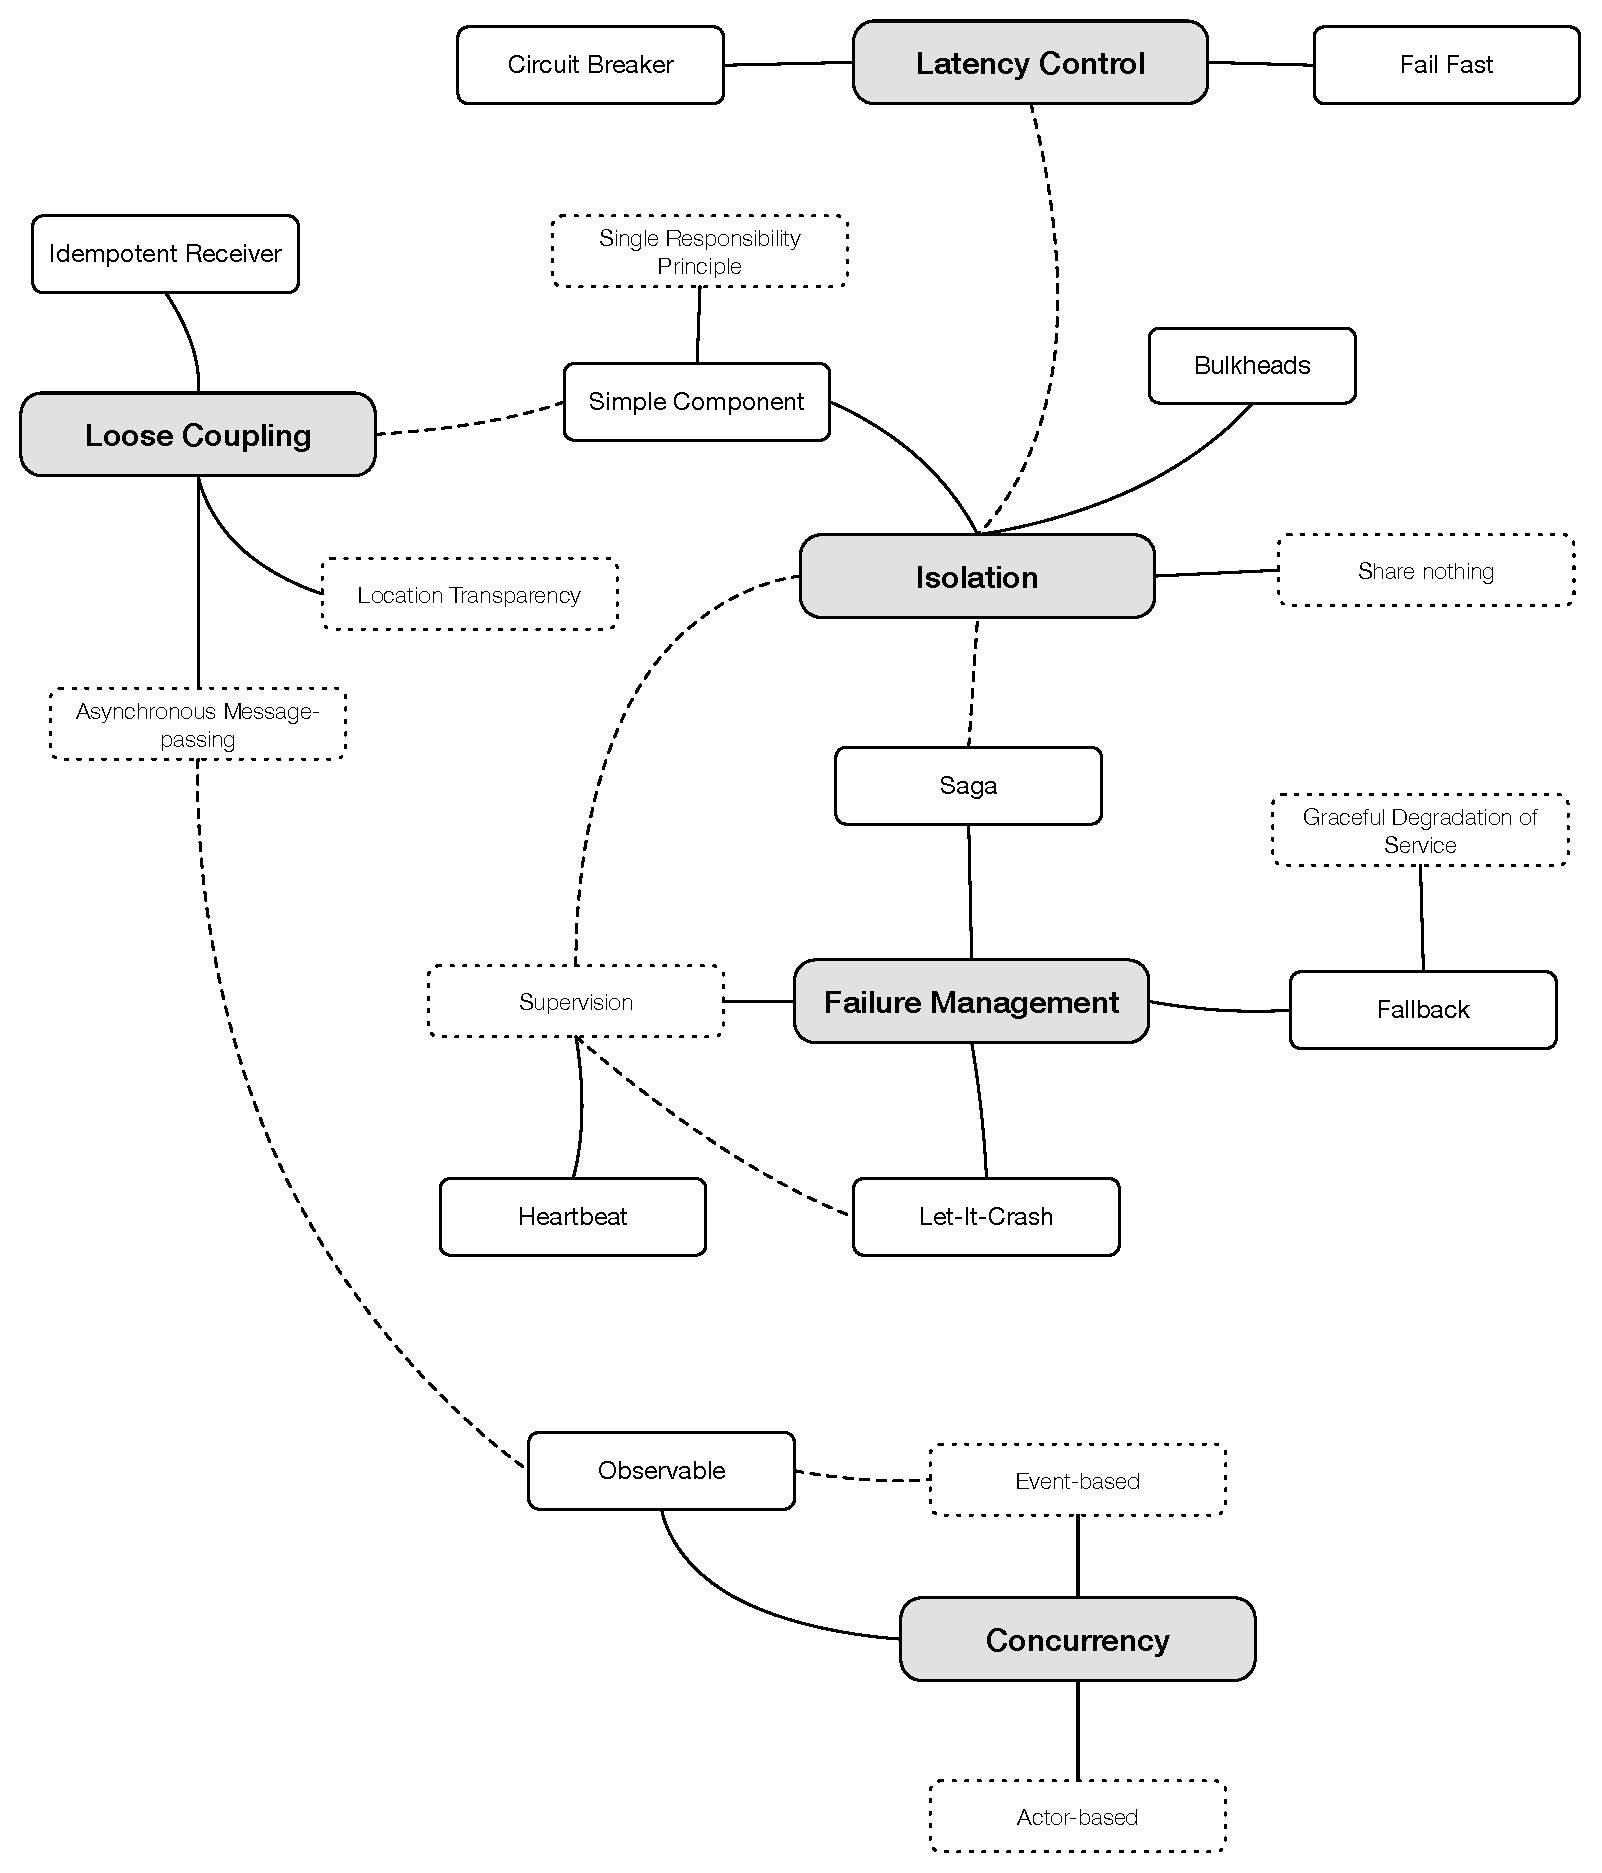
\includegraphics[width=0.9\textwidth]{4-Hauptteil/context/context.eps}
 \caption{Reactive Design Pattern und weitere Eigenschaften im Kontext.}
 \label{fig:patterns-context}
\end{figure}